\section{Testing}
\label{testing}

We measured the execution time and RAM usage of our three Mini-MAC implementations 
running on the Texas Instruments MSP430F5529 microcontroller. 
In speed and power this device is representative of vehicular ECUs.

\subsection{Purpose}
\label{purpose}

The purpose of our tests is to measure the time and space usage of our Mini-MAC implementations, and more generally,
to evaluate the performance suitability of Mini-MAC for authenticating messages on the CAN bus.

\subsection{Methods}
\label{methods}

For each implementation we measured code size, memory usage, execution time, and bus utilization,
collecting for each implementation metrics from 1000 inputs of various typical sizes (1~byte, 2~bytes, 4~bytes).  

We measured code size and RAM usage at compile time using 
the Texas Instruments Code Composer v6.
The RAM usage is known at compile time because there is no
dynamic memory allocation.

We measured execution time using a counter register on the MSP430 running at 8 MHz. The 32 kHz external clock on the test board provides timing values to approximate millisecond~(ms) accuracy.
As a very minor point we note that, due to a limitation in the hardware's
support for timing measurements, 
there may be a $\pm$0.03~ms inaccuracy in each reading due to the
time it takes to read the counter.

We collected statistics on message traffic from a 2010 Toyota Prius with a CAN-bus sniffer program 
based on an Arduino Uno platform and connected via an OBD-II CAN transceiver shield.
	
	\begin{table}
	\centering
	\caption{Additional bus traffic for various authentication mechanisms, 
	for one key group with $n$ recipients.  Mini-MAC adds no additional bus traffic}
	\label{tab-traffic}
	\vspace{8pt}
	\begin{tabular}{l|r}%
	\bfseries Algorithm & \bfseries Additional \\
	& {\bf Traffic (bits)} \\\hline 
	HMAC-MD5 (Group) & 128 \\
	HMAC-MD5 (Pairwise) & 128$n$ \\
	Lin-MAC & 128$n$ \\
	Mini-MAC & 0 \\
	\end{tabular}
	\end{table}

\begin{table}	
	\centering	
	\caption{Additional code size and mean additional time to compute Mini-MAC implementations over HMAC.
	For each implementation, the additional RAM usage is 5~bytes.}
	\label{tab-overhead}
	\vspace{8pt}
	\begin{tabular}{l|c|c}
	\bfseries Hash & \bfseries Code Size  & \bfseries Execution\\
	& \bfseries (bytes) & \bfseries Time (ms)\\\hline 
	MD5 & 835 & 0.38 \\
	SHA-1 & 850 & 0.42 \\
	SHA-2 & 766 & 0.68 \\
	\end{tabular}
	\end{table}
	
	\begin{table}
	\centering
	\caption{Execution time (observed mean $\pm$ standard deviation) of Mini-MAC implementations.
	Only the MD5 implementation meets our engineering requirement of at most 25~ms per message.}
	\label{tab-time}
	\vspace{8pt}
	\begin{tabular}{ @{}l | rcl}
	\hspace{2pt}\textbf{Hash} && {\textbf{Time (ms)}}&\\
		& $\mu$ & $\pm$ & $\sigma$   \\
		\hline 
		\hspace{2pt}MD5 	& 7.5 		& $\pm$ 	& 0.07 \\
		\hspace{2pt}SHA-1 	& 28.0 		& $\pm$		& 0.06 \\
		\hspace{2pt}SHA-2 	& 69.6 		& $\pm$		& 0.08 \\ 
	\end{tabular}	
	\end{table}
	
	\begin{figure}
		\centering
		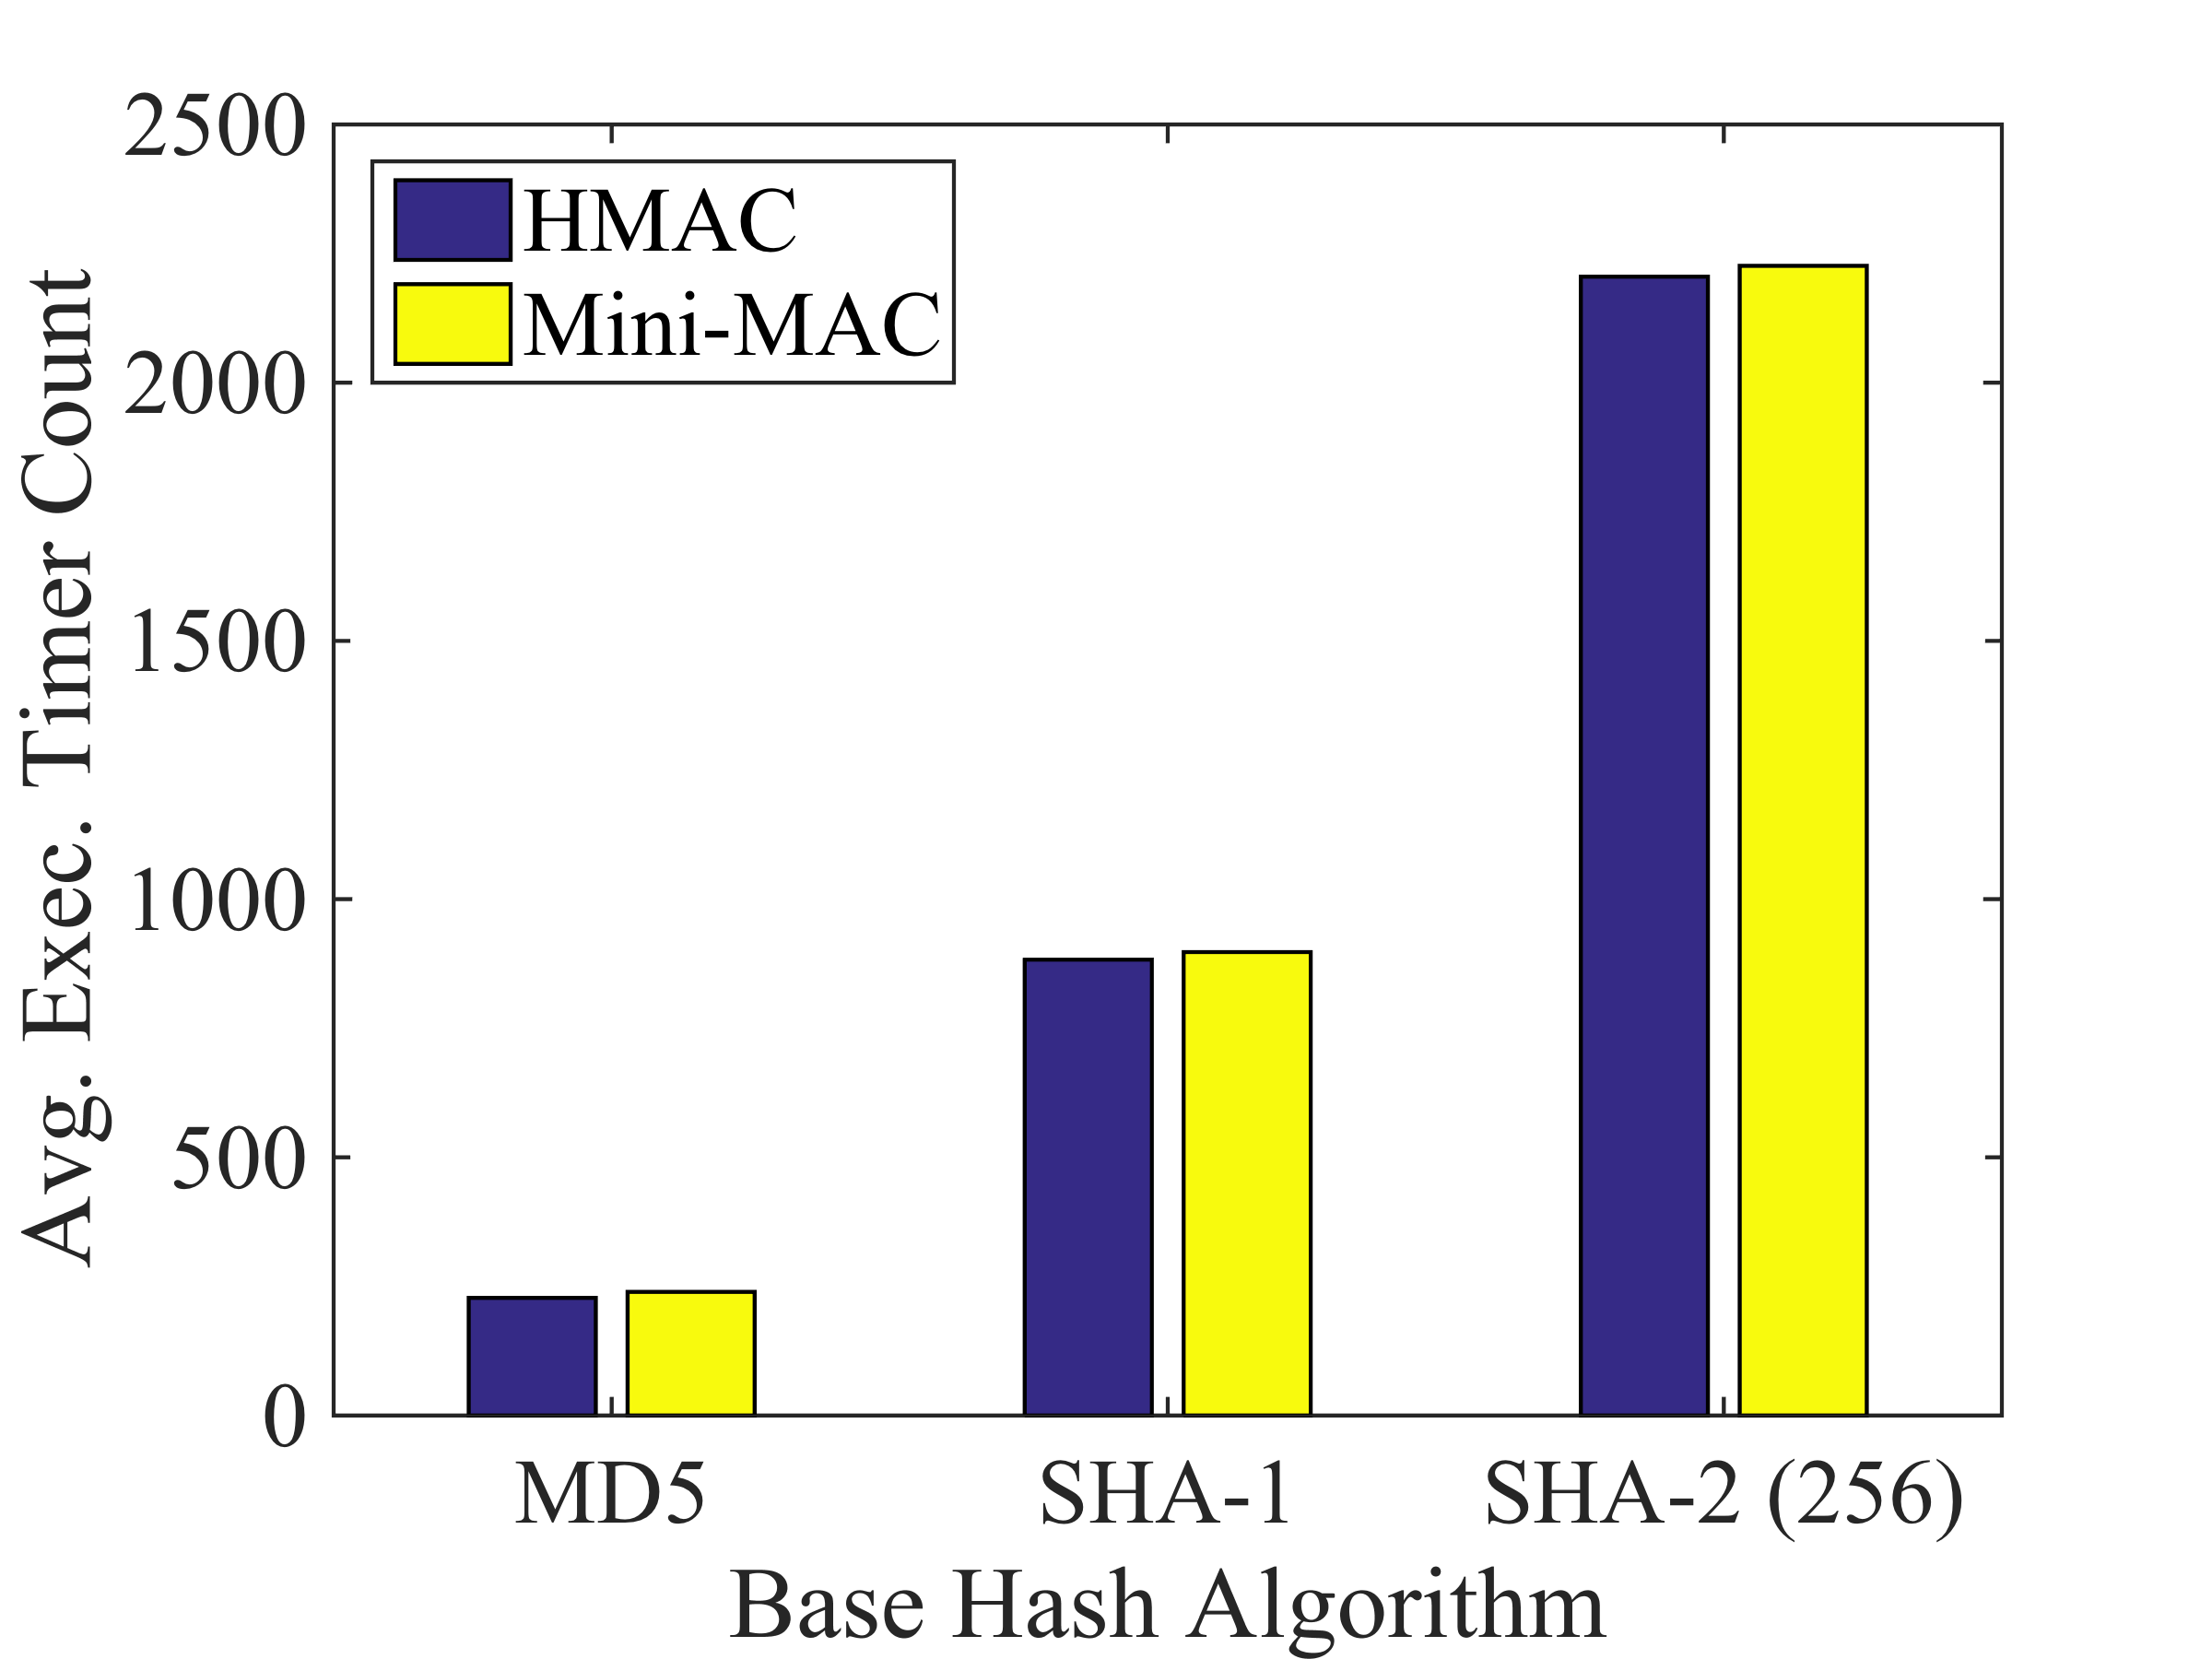
\includegraphics[width=\columnwidth]{figures/exec_cycles.png}
		\caption{Mean execution time for our Mini-MAC implementations, in cycles on a 32~kHz clock,
		from 1000 messages.}
		\label{fig-execution}
	\end{figure}
	
	\begin{figure}
		\centering
		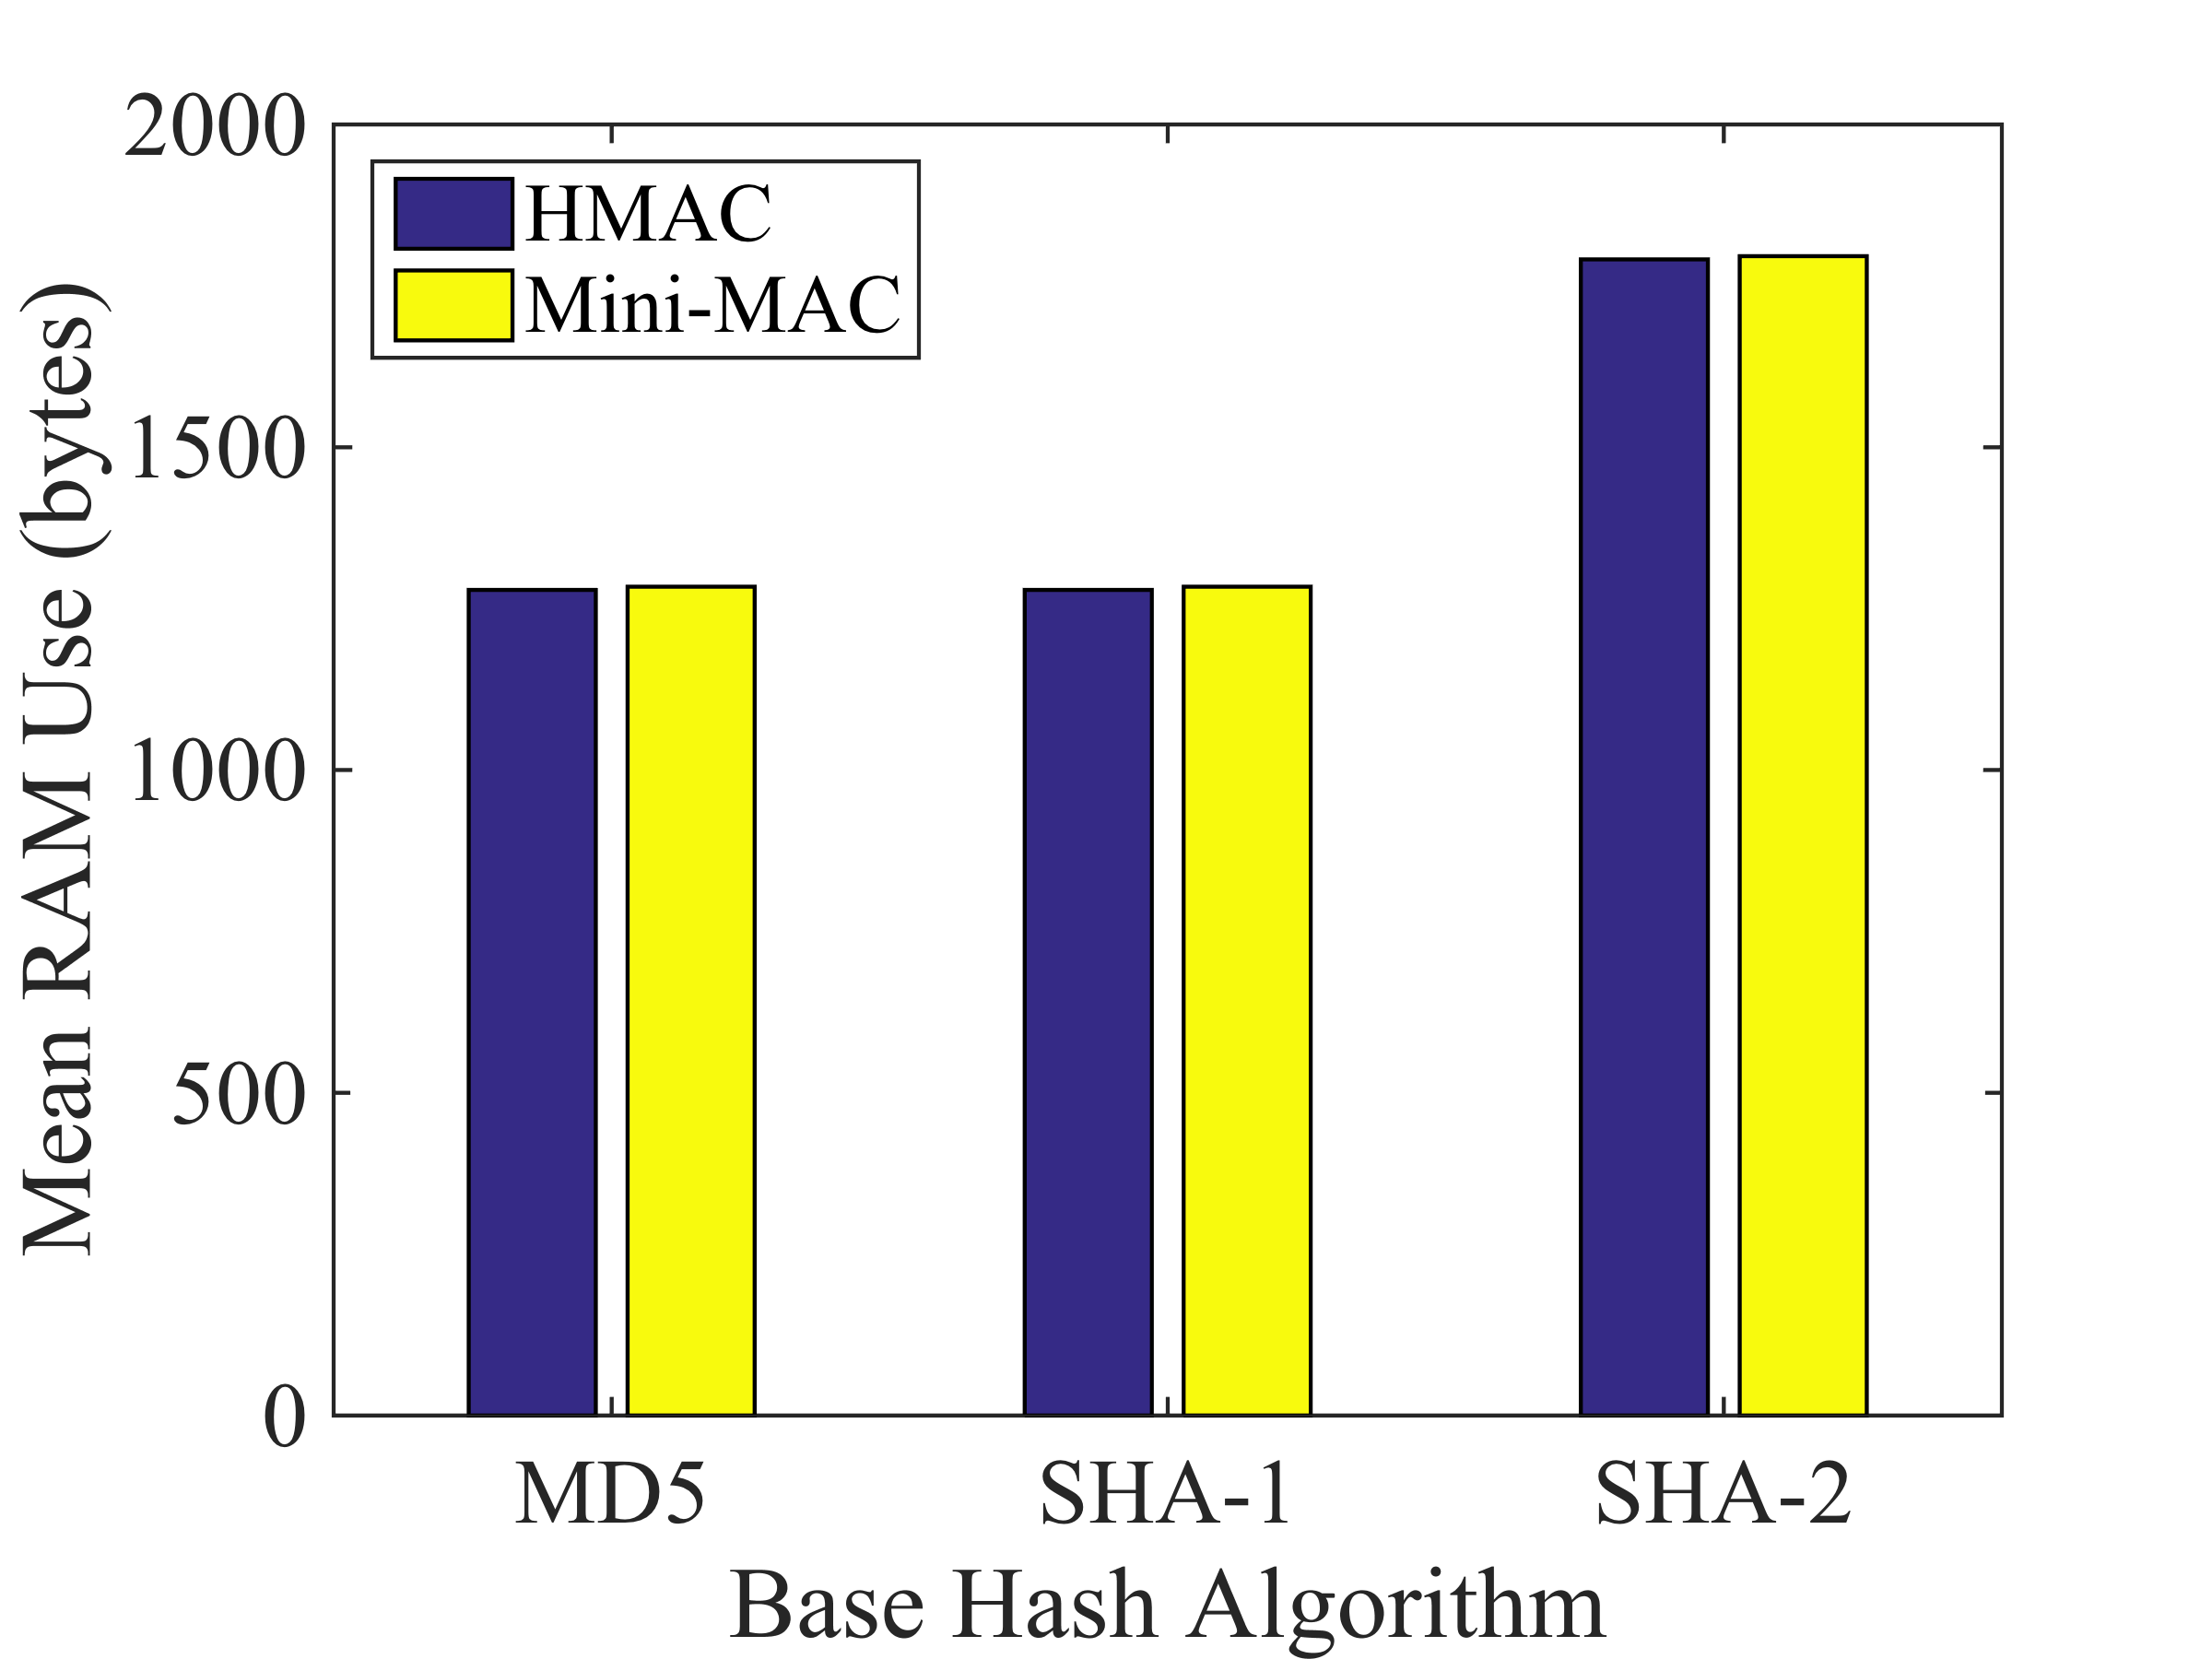
\includegraphics[width=\columnwidth]{figures/ram_usage.png}
		\caption{RAM usage for our Mini-MAC implementations, from 1000 messages.}
		\label{fig-ram}
	\end{figure}
	
	\begin{figure}
		\centering
		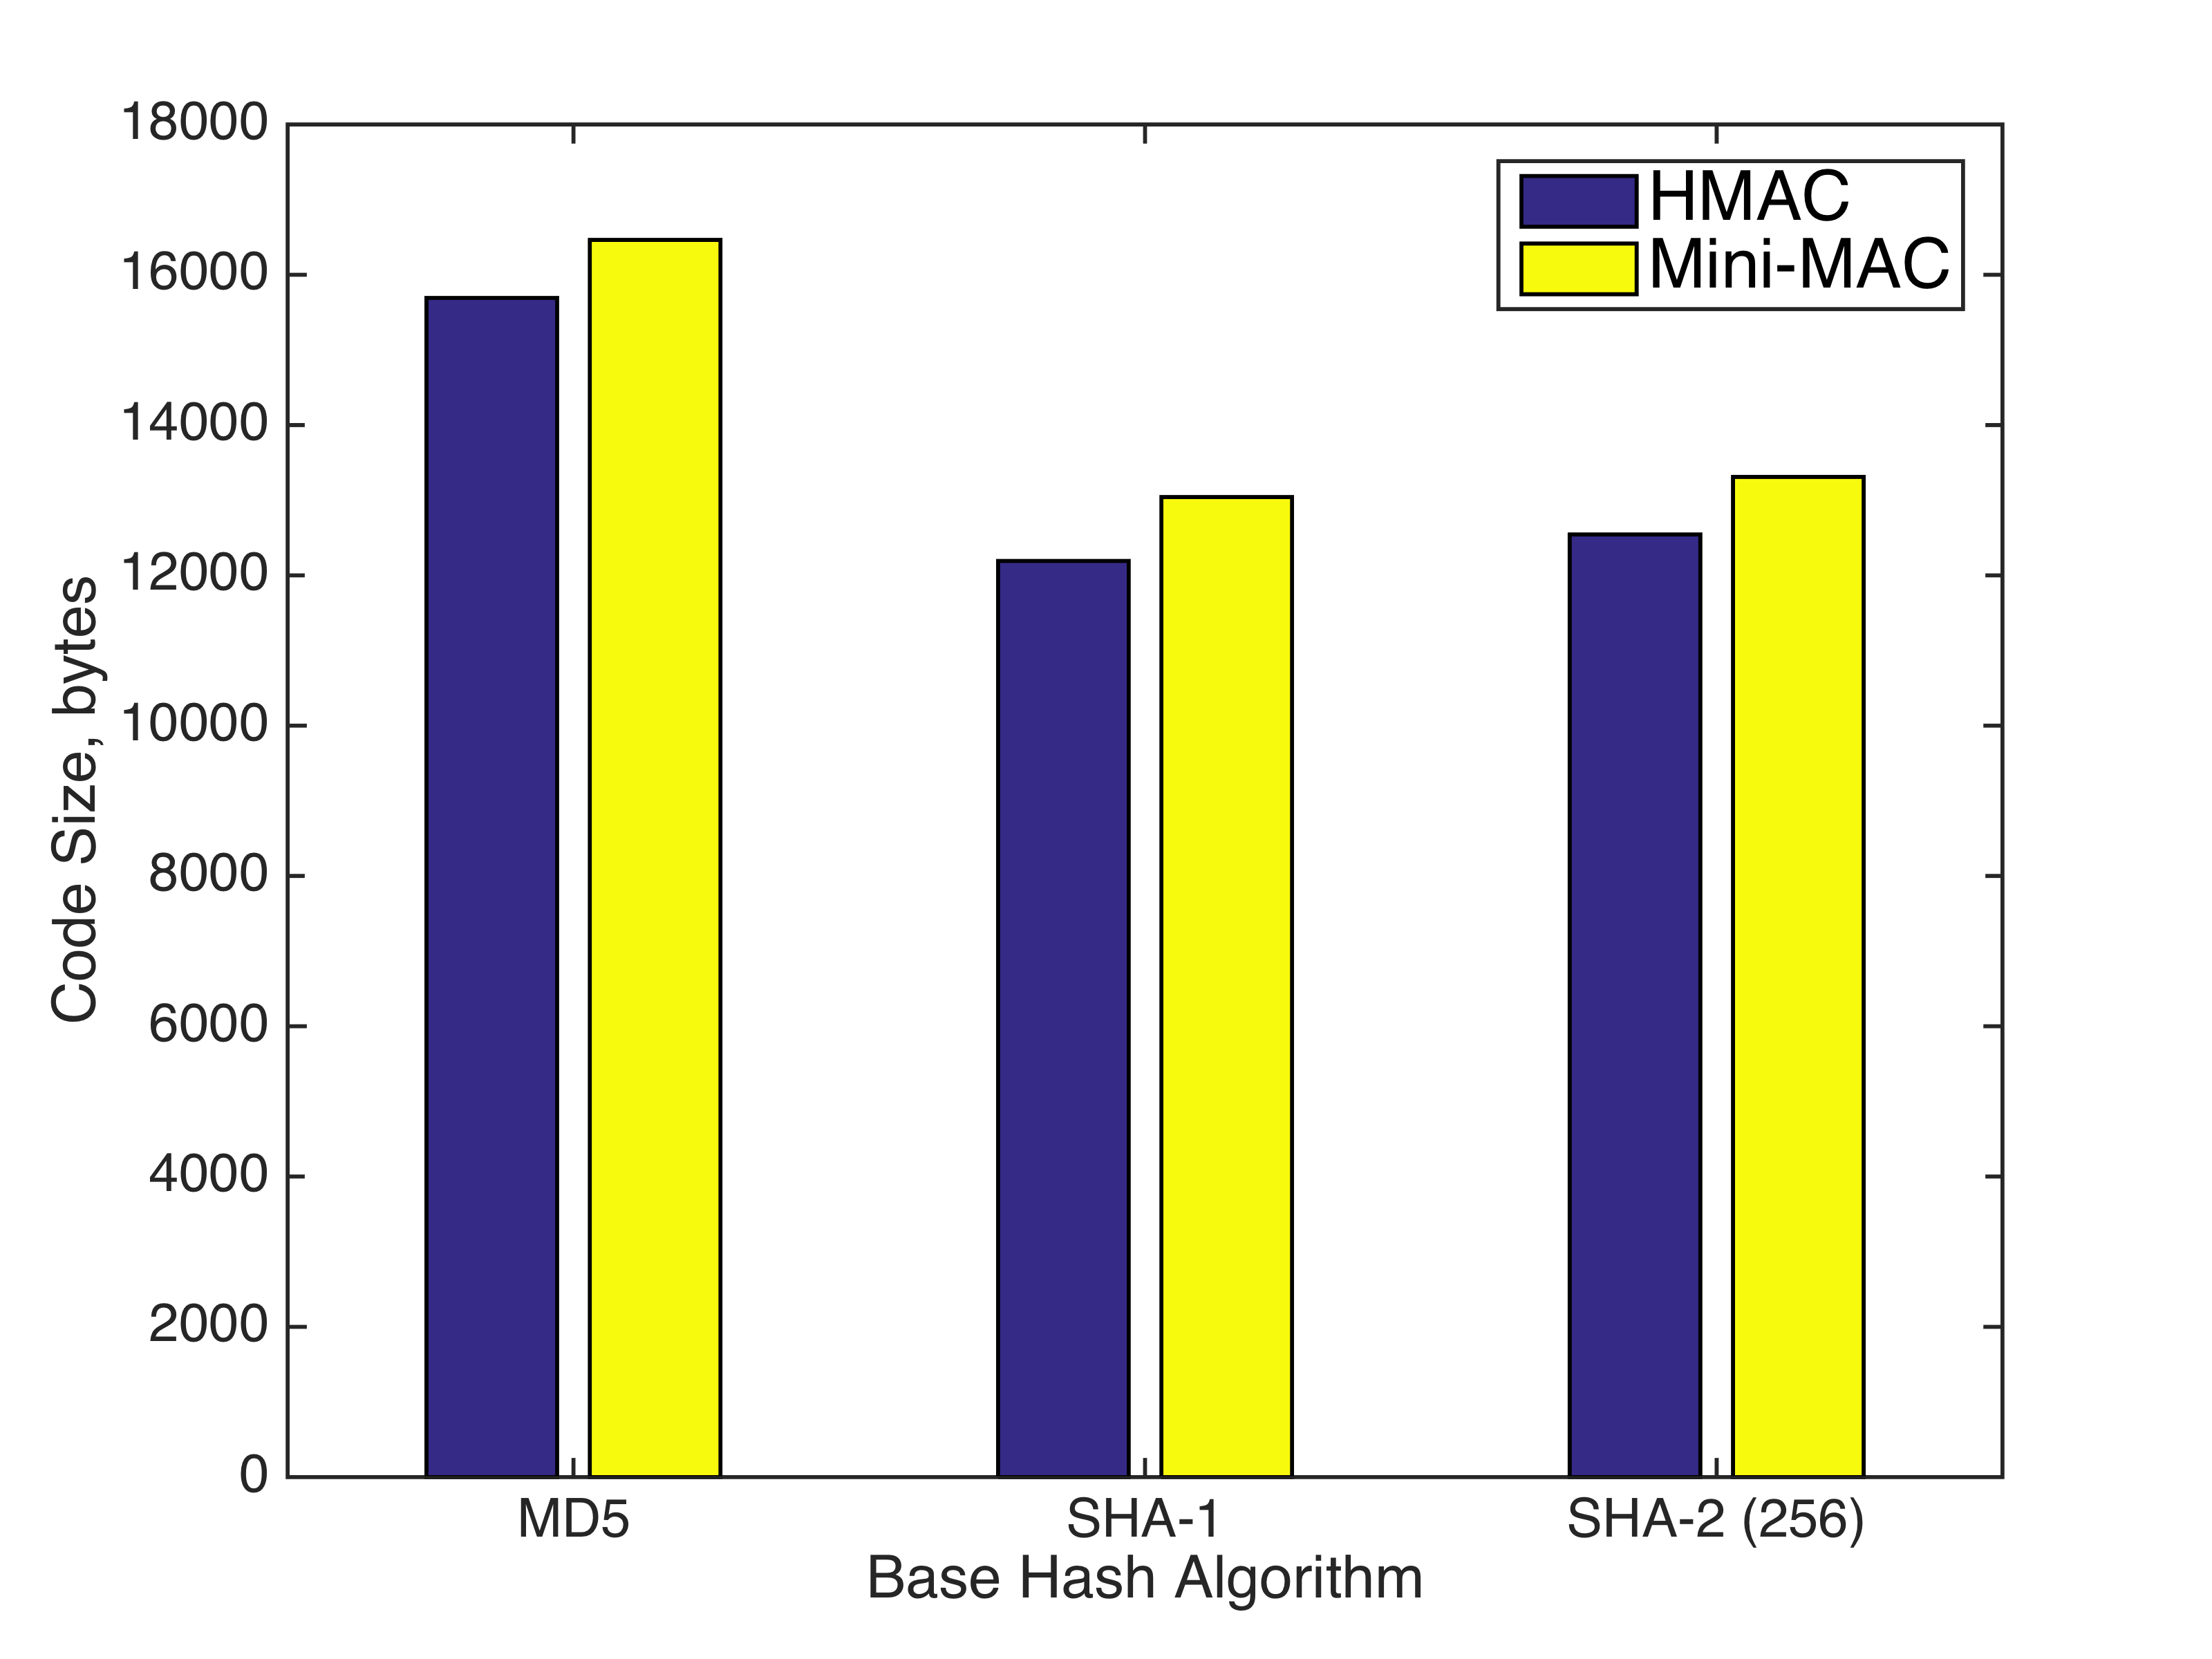
\includegraphics[width=\columnwidth]{figures/code_size.png}
		\caption{Code size of our Mini-MAC implementations.}
		\label{fig-code}
	\end{figure}
	
	
	